\documentclass[twoside]{article}

\usepackage{epsfig}
\usepackage{amsfonts}
\usepackage{tikz}

\setlength{\oddsidemargin}{0.25 in}
\setlength{\evensidemargin}{-0.25 in}
\setlength{\topmargin}{-0.6 in}
\setlength{\textwidth}{6.5 in}
\setlength{\textheight}{8.5 in}
\setlength{\headsep}{0.75 in}
\setlength{\parindent}{0 in}
\setlength{\parskip}{0.1 in}

\newcommand{\lecture}[4]{
   \pagestyle{myheadings}
   \thispagestyle{plain}
   \newpage
   \setcounter{page}{1}
   \noindent
   \begin{center}
   \framebox{
      \vbox{\vspace{2mm}
    \hbox to 6.28in { {\bf STA561:~Probabilistic machine learning \hfill} }
       \vspace{6mm}
       \hbox to 6.28in { {\Large \hfill #1 (#2)  \hfill} }
       \vspace{6mm}
       \hbox to 6.28in { {\it Lecturer: #3 \hfill Scribes: #4} }
      \vspace{2mm}}
   }
   \end{center}
   \markboth{#1}{#1}
   \vspace*{4mm}
}

\begin{document}

\lecture{Variational Inference}{11/4/13}{Barbara Engelhardt}{Tracy Schifeling, Alireza Samany, and Matt Dickenson}

\section{Introduction}


\section{Ising Model}

% previous section should end with a discussion of ELBO
Before proceeding with variational inference, it is helpful to review the Ising model. The main idea behind the Ising model is a lattice of unobserved variables ($x_1,...x_n$), each with its own (noisy) observation ($y_1, ..., y_n)$). 

For example, suppose our goal is to reconstruct a denoised image given noisy observations of the pixels. We can think of the lattice as  the pixels in a black and white image ($x_i \in \{-1, 1\}$), with a noisy grayscale observation of the pixels ($y_i \in R)$. More generally, we wish to draw inferences about the unobserved lattice $X$ from the observed values $Y$. Figure \ref{ising} illustrates an Ising model for $n=9$, with the latent nodes colored white and the observed nodes shaded grey. 

\begin{figure}[h!]
\begin{center}
\begin{tikzpicture}
\scriptsize
\foreach \i in {1,...,9}
{
        \pgfmathtruncatemacro{\y}{(\i - 1) / 3};
        \pgfmathtruncatemacro{\x}{\i - 3 * \y};
        \pgfmathtruncatemacro{\label}{\x + 3 * (2 - \y)};
        \pgfmathtruncatemacro{\labely}{(\x + 3 * (2 - \y))*10};
        \node[circle,draw=black,fill=white,minimum size=20]
        (\label) at (1.5*\x,1.5*\y) {$x_\label$};
        \node[circle,draw=black,fill=white!80!black,minimum size=20]
        (\labely) at (1.5*\x-0.8,1.5*\y-0.8) {$y_\label$};
}
% Lattice of X's
\draw (1) -- (2);
\draw (1) -- (4);
\draw (2) -- (3);
\draw (2) -- (5);
\draw (3) -- (6);
\draw (4) -- (5);
\draw (4) -- (7);
\draw (5) -- (6);
\draw (5) -- (8);
\draw (6) -- (9);
\draw (7) -- (8);
\draw (8) -- (9);
% X to Y
\draw (1) -- (10);
\draw (2) -- (20);
\draw (3) -- (30);
\draw (4) -- (40);
\draw (5) -- (50);
\draw (6) -- (60);
\draw (7) -- (70);
\draw (8) -- (80);
\draw (9) -- (90);
\end{tikzpicture} 
\end{center}
\caption{Schematic of an Ising Model}
\label{ising}
\end{figure}

We now define the potential functions of the Ising model:
\begin{eqnarray*}
\psi_s(x_s) &=& p(y_i | x_i) \equiv L_i(x_i) \\
\psi_{st} (x_s x_t) &=& W_{st} x_s x_t 
\end{eqnarray*} 
Continuing with our image example above, we could set $W_{st}=1$. In general, we set $W$ to positive values if we want neighbors to agree, and negative values if we want them to differ. 

Let $N(i)$ be a function that returns the first-degree neighbors of node $i$. For example, in Figure \ref{ising}, calling $N(x_1)$ would return nodes $x_2$ and $x_4$.

Now we can specify functions for our prior:
\begin{eqnarray*}
p(x) &=& {1 \over z_0} \exp\{ - \sum_{i=1}^n \sum_{j \in N(i)} x_i x_j \} \\
p(y|x) &=& \prod_{i=1}^n \exp \{-L_i(x_i) \} 
\end{eqnarray*}

From this, we have the posterior:
\begin{eqnarray*}
p(x|y) &=& {1 \over z} \exp \{ - \sum_{i=1}^n  \sum_{j \in N(i)} x_i x_j - \sum_{i=1}^n L_i(x_i) \}
\end{eqnarray*}

\subsection{Mean Field Version of the Ising Model}

Having seen an example of a basic Ising model, we now turn our attention to how we can analyze the mean field version of such a model. We do this by ``breaking'' the edges between the latent variables. We add a mean value (or variational parameter) $\mu$ to each $x$, such that $\mu_i=\mathbb{E}[x_i]$. The new structure is illustrated in Figure \ref{meanfield}, with the same color coding as above. 

\begin{figure}[h!]
\begin{center}
\begin{tikzpicture}
\scriptsize
\foreach \i in {1,...,3}
{
        \pgfmathtruncatemacro{\y}{(\i - 1) / 3};
        \pgfmathtruncatemacro{\x}{\i - 3 * \y};
        \pgfmathtruncatemacro{\label}{\x};
        \pgfmathtruncatemacro{\labely}{\x*10};
        \pgfmathtruncatemacro{\labelm}{\x*100};
        \node[circle,draw=black,fill=white,minimum size=20]
        (\label) at (1.5*\x,1.5*\y) {$x_\label$};
        \node[circle,draw=black,fill=white!80!black,minimum size=20]
        (\labely) at (1.5*\x-0.8,1.5*\y-0.8) {$y_\label$};
        \node[circle,draw=black,fill=white,minimum size=20]
        (\labelm) at (1.5*\x+0.8,1.5*\y+0.8) {$\mu_\label$};
}
\draw (1) -- (10);
\draw (2) -- (20);
\draw (3) -- (30);
\draw (1) -- (100);
\draw (2) -- (200);
\draw (3) -- (300);
\end{tikzpicture} 
\end{center}
\caption{Mean Field Version of an Ising Model}
\label{meanfield}
\end{figure}


% todo: explain what q is/where it comes from
\begin{eqnarray*}
q(x) &=& \prod_{i=1}^n q_i (x_i) \\
\log ( q_i (x_i)) &=& \mathbb{E}_q [ \log \tilde{p}(x) ]
\end{eqnarray*}

We can maximize $\log ( q_i (x_i))$ with a coordinate ascent method, as discussed previously in class.

Now, we rewrite the ELBO in terms of the Ising model:
\begin{eqnarray*}
\log (q_i (x_i)) &=& \mathbb{E}_{q_i} [ x_i \sum_{j \in N(i)} x_j + L_i(x_i) +c ] \\
q_i (x_i) &\propto& \exp \{ x_i \sum_{j \in N(i)} \mu_j + L_i(x_i) \}
\end{eqnarray*}
% propto line may not be correct

Thus, 
\begin{eqnarray*}
q_i(x_i=+1) &=& { \exp\{ \sum_{j \in N(i)} \mu_j + L_i(+1) \}   \over \sum_{x_i^{\prime} \in \{ +1, -1\}} \exp \{ \sum_{j \in N(i)} \mu_j + L_i(x_i^{\prime}) \} }
\end{eqnarray*}
Note the resemblance of this function to a sigmoid function $1 \over 1+q_i(x_i=-1)$. Effectively, this $q_i$ is an approximation of the marginalized posterior, or basically a Gibbs step.

For the mean field, we now iteratively updateL 
\begin{eqnarray*}
mu_i = +1 (q_i(x_i=+1)) + -1 (q_i(x_i=-1)) \\
z_i \propto \exp[ \mathbb{E}[ \log p(z|x)]]
\end{eqnarray*}

In the model, we have three parameters of interest: $\mu_1, \mu_2$, and $\mu_{12}$, where $\mu_{12}=\mathbb{E}[\psi_{12}(x_1 x_2)]$. We have the constraint $0 \leq \mu_{12} \leq \mu_1, \mu_2$. We limit acceptable values to those within the portion of the simplex that satisfies this constraint. 

% insert a picture

If we take a slice of this convex polytope, it is a trinagle. % some more stuff here

\section{Loopy Belief Propogation}



\end{document}

